\begin{figure}[t]
    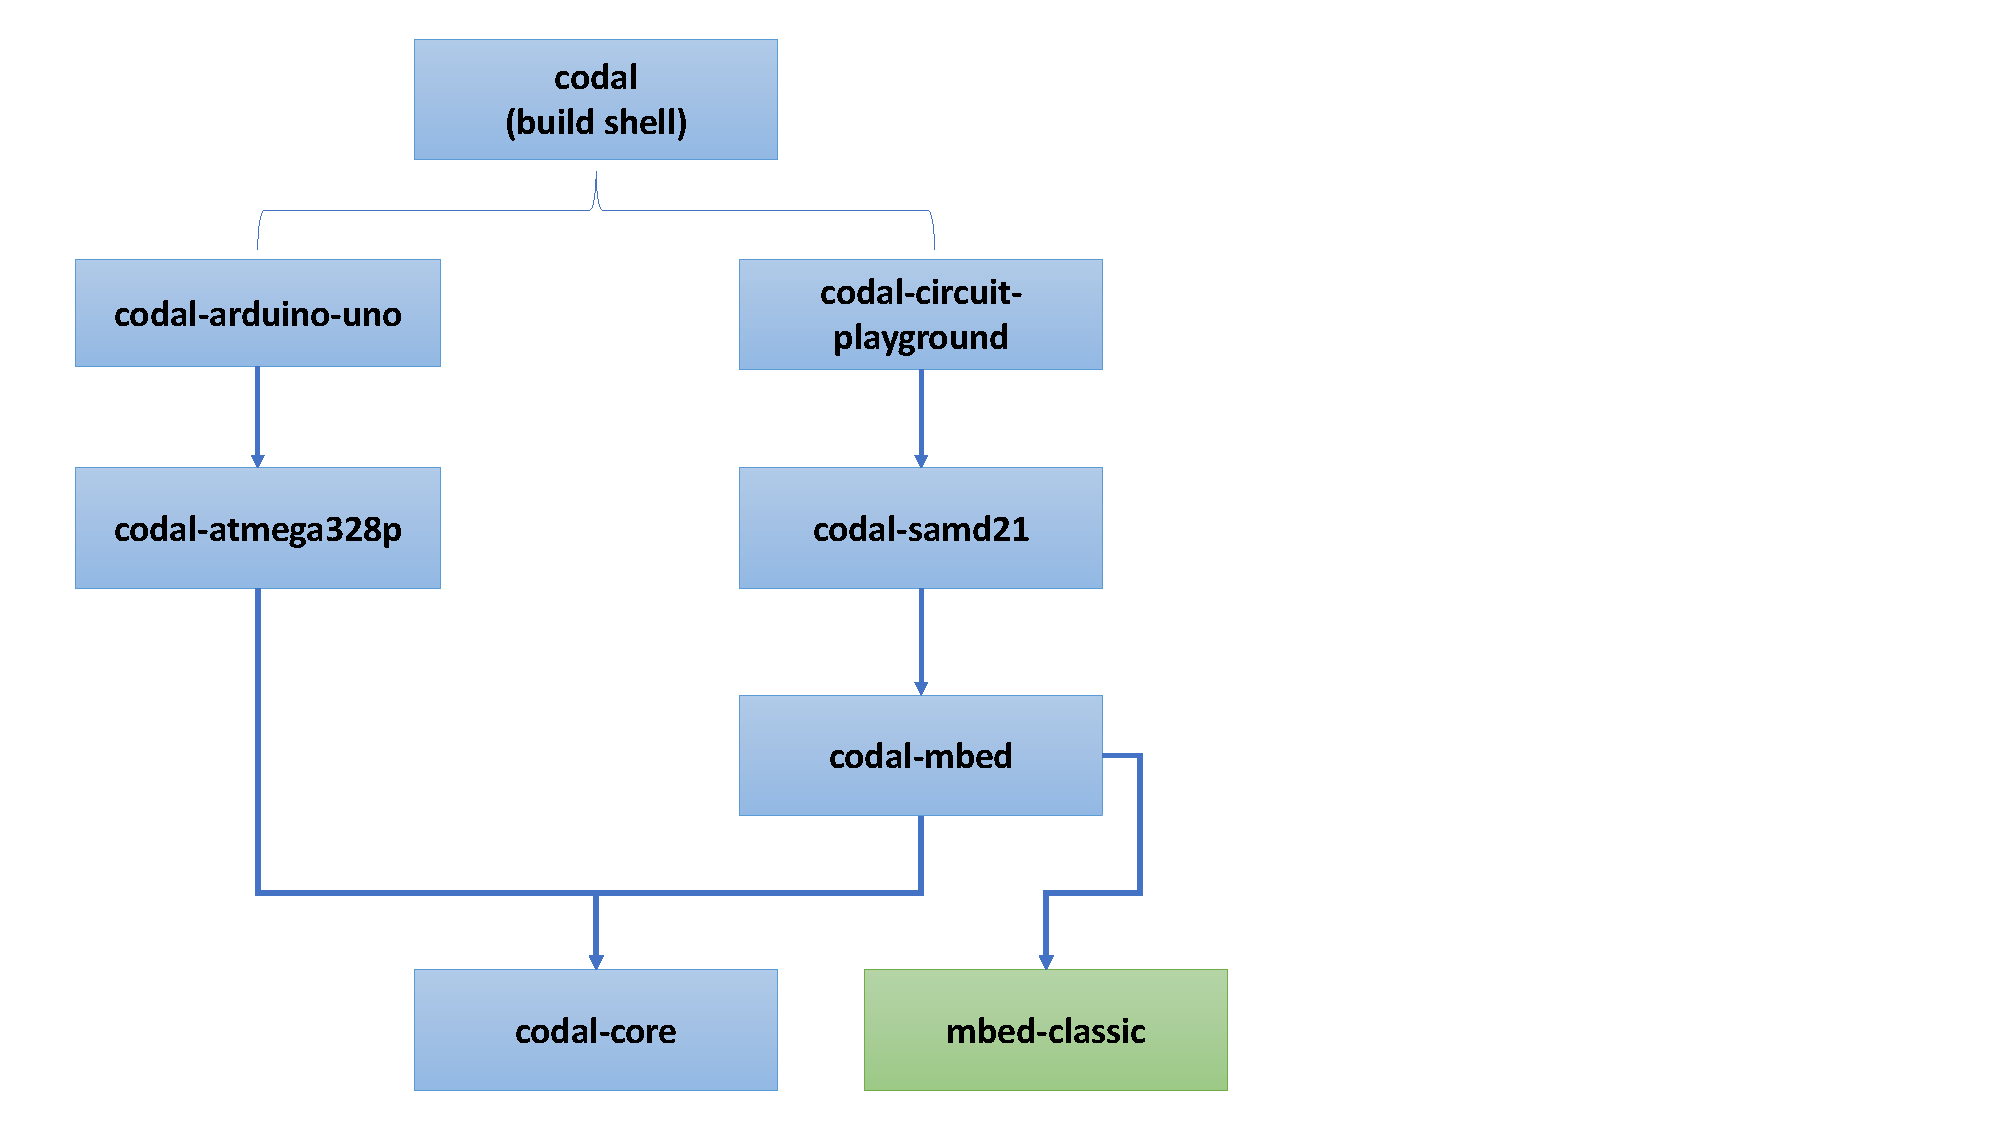
\includegraphics[width=4.5in]{codalFig.pdf}
    \caption{\label{fig:codal}Detailed relationships between CODAL repos.}
\end{figure}

\section{The CODAL Runtime}
\label{sec:codal}

Typically written in C and/or C++, platforms for microcontroller programming all share a common design goal: to support developers by providing primitives and programming abstractions. Platforms can range from simple C++ classes that control hardware, to real-time operating systems (RTOSs) with scheduling and memory management.

The Arduino ecosystem is an example of a simple platform where the developer uses high-level APIs to control hardware; there is no scheduler, and memory management is discouraged through a heavy emphasis on global variables.  The Arduino programming model is based on polling: an Arduino ``sketch'' is a program template that consists of a setup procedure, for initialization of data structures, and a loop procedure; programmers implement the body of \textit{setup} and \textit{loop}, where they explicitly poll the state of the sensors or the microcontroller's pins.

At the other end of the spectrum is mbed OS, which is aimed at developers who are familiar with non-preemptive scheduling, memory management, and condition synchronisation; a more complex environment. A number of high-level drivers are provided and the programming model is determined by the developer, commonly event or interrupt driven.

Although platforms like Arduino and mbed OS are widely used by C/C++ developers, higher-level languages opt for virtual machines to execute on microcontrollers as neither extreme aligns with the programming models seen in higher level languages: mbed OS is pre-emptive, JavaScript is not; Arduino is based on monolithic polling. There is therefore a need to develop a layer that: (1) bridges the semantic gap between the higher-level language and the hardware; (2) does so in a memory, energy and instruction efficient way; and (3) supports a number of platforms with various resource contraints and capabilities.

\subsection{Codal}

The component-oriented device abstraction layer (CODAL) aims to provide a layer that is multi-platform, makes efficient use of memory and energy, provides both synchronous and asynchronous API variants, and offers a good experience for native C and higher level languages.

CODAL provides a set of components that abstract away microcontroller specifics, a non-preemptive scheduler that minimises the need for resource locking primitives whilst allowing asynchronous operation, and an eventing subsystem common to all CODAL Components that enables the decoupling of system and user code. A CODAL component represents software or hardware drivers (an I2C device, a GPIO pin, a Message Bus, a Bluetooth device); any component can generate or consume events. CODAL supports both polling and asynchronous (event-driven) programming models, which enables higher level languages to map straight onto native C/C++ APIs.

Unlike mbed, which is designed to make all devices look programmatically alike, CODAL enables devices with additional on-chip hardware to specialise device drivers with APIs that can then be used by the end application developer.

% more required here, needs to be reflowed...

\subsubsection{Structural Overview}

* a nice diagram
* an object model that factors out common code, but pushes platform specific code.
* why it's required:
    - platform independence
    - extensibility
    - platform specialisation
* explanation
Worked example of how everything fits together, short, only a few sentences.

* the core
* the targets
* supporting library

\subsubsection{Message Bus and Events}

Message passing via events is a common technique and is the foundation of many operating systems --- yet in most systems events are static used only to notify users of key events within the system (e.g. SIGKILL on UNIX).

In CODAL, we offer extensible events where the data contained in an event can be arbitrary, commonly application specific. Application developers can then ``listen'' to events, specifying an id (namespace), a value (unique within a namespace), and a function to be invoked when an event is raised. Events pass through the message bus, if a corresponding listener is in place, the function indicated by the listener is invoked. The eventing model aligns well to languages like JavaScript as well as Scratch blocks such as ``on button pressed''. An example is given below:

\begin{lstlisting}
#include "CircuitPlayground.h"
CircuitPlayground cplay;

void a_listener() { // do something }

int main() {
    cplay.messageBus.listen(100,100,a_listener);
    Event(100,100);
}
\end{lstlisting}

Not only do events enable easy modularisation of code, but they also safeguard the application programmer from situations where incorrect code could cause unexpected behaviour. Take for example an application to detect a button press, there are usually two solutions: (1) poll the state of a pin; or (2) configure an interrupt to fire when the state of a pin changes. Taking the latter approach, it could look something like this:

\begin{lstlisting}
int state = 0;

void buttonClicked() {
    int gpioState = PIN0;
    // button released, blink LED!
    if(state == 1 && gpioState == 0) {
        set_state(LED, 1);
        wait_ms(1000);
        set_state(LED, 0);
    }
    state = gpioState;
}

int main() {
    configure_interrupt(PIN0, buttonClicked);
    while(1);
}
\end{lstlisting}

The above code sample is considered bad practice as it prevents other interrupts (like Timers) from firing for at least a second when a button is released, however, this is often the first application that a user will create. Such frameworks advise users to avoid blocking functions and waiting in interrupt context, thus sidestepping the problem by punting responsibility to the user --- CODAL uses the message bus abstraction to shield users from such scenarios:

\begin{lstlisting}
#include "CircuitPlayground.h"
CircuitPlayground cplay;

void buttonClicked() {
    cplay.io.led.setDigitalValue(1);
    cplay.sleep(1000);
    cplay.io.led.setDigitalValue(0);
}

int main() {
    cplay.messageBus.listen(ID_BUTTON_A,DEVICE_BUTTON_EVT_CLICK,buttonClicked);

    while(1) cplay.sleep(100);
}
\end{lstlisting}

Note that the user doesn't have to configure any interrupts, as they are handled by pre-existing drivers.

% Stuff to add (it's already quite long):
% * Provides a similar mechanism seen in higher level languages
% * Timer and queues?
% * message passing microkernel

\subsubsection{Fiber Scheduler}

Novice users often want to perform multiple operations concurrently, generally requiring threads. Threading is a confusing concept: users have to learn about locks, semaphores, and preemption, to prevent race conditions. Threads can also consume a large number of resources depending on the model that is adopted by the runtime environment.

CODAL takes a non-preemptive scheduling approach which reduces the need for resource locking primitives. In CODAL's scheduling model, fibers (a lightweight thread) are RAM efficient and are only paged out when a user explicitly calls ``sleep'', meaning that the stack depth at the point where a fiber is paged out is small. Fibers have a variable stack size, and when paged out the entire stack is duplicated to the heap --- this would normally be ill-advised, but due to a usually small stack size, this is more efficient than approaches where there is a mandated stack size.

Events and the message bus are integral to CODAL even extending to fibers, which can block and wait on events to complete:

\begin{lstlisting}
#include "CircuitPlayground.h"
CircuitPlayground cplay;

void block() {
    // block the calling thread until the user clicks button a!
    fiber_wake_on_event(ID_BUTTON_A,DEVICE_BUTTON_EVT_CLICK,buttonClicked);
    cplay.io.led.setDigitalValue(1);
}

int main() {
    create_fiber(block);
    // wait until the button
    fiber_wait_for_event(ID_BUTTON_A,DEVICE_BUTTON_EVT_CLICK,buttonClicked);
    cplay.io.led.setDigitalValue(0);
}
\end{lstlisting}

\subsubsection{Drivers}

Drivers are commonly low level interfaces that control external or integrated hardware on a device. For embedded developers, creating and using drivers involves translating datasheets into program code and using low-level interface, which can alienate novice programmers.

In CODAL, drivers abstract away the complexities of the underlying hardware into reusable, extensible, easy-to-use components; for every hardware component there is a software component. There are three types of drivers in CODAL: (1) an abstract specification of a driver model common to most devices (e.g. I2C, Serial); (2) a driver that relies only on the interfaces specified in a driver model  (e.g. an I2C based device); and (3) the concrete implementation of the abstract driver model, which may be platform specific or platform agnostic. Not all devices are the same, and by generalising the interface devices can introduce platform specific optimisations and specialisations.

Interrupts are integral to drivers: in Serial communications it is useful to know when a byte has been sent or received. As illustrated in the button example, performing operations in interrupt context can be detrimental to the device. CODAL drivers use events to decouple computational tasks, that may take a variable length of time, from interrupt context.

% * motivation
% * example - I2C, microphone (DMA)
% * one component per piece of hardware or software
% * Provides a common interface
% * uses events to decouple from interrupt context.

\subsubsection{Memory Management}

% * provides an interrupt safe environment for memory allocation
% * flexible implementation
%     - multiple heaps
%     - reconfigurable, repurposeable
% * optimisations for common sizes and repeated patterns
% * edu
% * couple of sentences on types
%     - ref counted, malloced types.

\subsubsection{Streams}

% * motivation
% * example
% * Pull and Push model
% * Adopted by all stream capable interfaces, from Serial to I2C
% * Worked example, audio recog, playback

\subsubsection{A code sample}

% * That says this is awesome!
% * how it fits together...

\subsection{Evaluation}

% - Profile fibers, how much do they actually use? are they any better?
%     - average RAM consumption for X
%     - Stack is typically small...
%     - types aid the stack size (heap allocated)
% - Compare memory allocator to lib c? (probably not that interesting)
% - benefits of componentisation?
%     - reusability, extensibility
% - How well does \MC + codal perform on each device? (SAMD, ATMEGA, NRF52)
%     - \MC + codal, native codal, mbed.
%     - cost benefit analysis of each.
%     - memory (flash and RAM) consumption
%     - CPU cycles
%         - context switch
%         - cost of events
%         - code gen, compare against micropython / espruino
%     - energy efficiency
%         - environmental sensing across 3 different platforms, mbed, espruino, codal